% Options for packages loaded elsewhere
\PassOptionsToPackage{unicode}{hyperref}
\PassOptionsToPackage{hyphens}{url}
%
\documentclass[
]{article}
\usepackage{amsmath,amssymb}
\usepackage{iftex}
\ifPDFTeX
  \usepackage[T1]{fontenc}
  \usepackage[utf8]{inputenc}
  \usepackage{textcomp} % provide euro and other symbols
\else % if luatex or xetex
  \usepackage{unicode-math} % this also loads fontspec
  \defaultfontfeatures{Scale=MatchLowercase}
  \defaultfontfeatures[\rmfamily]{Ligatures=TeX,Scale=1}
\fi
\usepackage{lmodern}
\ifPDFTeX\else
  % xetex/luatex font selection
\fi
% Use upquote if available, for straight quotes in verbatim environments
\IfFileExists{upquote.sty}{\usepackage{upquote}}{}
\IfFileExists{microtype.sty}{% use microtype if available
  \usepackage[]{microtype}
  \UseMicrotypeSet[protrusion]{basicmath} % disable protrusion for tt fonts
}{}
\makeatletter
\@ifundefined{KOMAClassName}{% if non-KOMA class
  \IfFileExists{parskip.sty}{%
    \usepackage{parskip}
  }{% else
    \setlength{\parindent}{0pt}
    \setlength{\parskip}{6pt plus 2pt minus 1pt}}
}{% if KOMA class
  \KOMAoptions{parskip=half}}
\makeatother
\usepackage{xcolor}
\usepackage[margin=1in]{geometry}
\usepackage{graphicx}
\makeatletter
\def\maxwidth{\ifdim\Gin@nat@width>\linewidth\linewidth\else\Gin@nat@width\fi}
\def\maxheight{\ifdim\Gin@nat@height>\textheight\textheight\else\Gin@nat@height\fi}
\makeatother
% Scale images if necessary, so that they will not overflow the page
% margins by default, and it is still possible to overwrite the defaults
% using explicit options in \includegraphics[width, height, ...]{}
\setkeys{Gin}{width=\maxwidth,height=\maxheight,keepaspectratio}
% Set default figure placement to htbp
\makeatletter
\def\fps@figure{htbp}
\makeatother
\setlength{\emergencystretch}{3em} % prevent overfull lines
\providecommand{\tightlist}{%
  \setlength{\itemsep}{0pt}\setlength{\parskip}{0pt}}
\setcounter{secnumdepth}{-\maxdimen} % remove section numbering
\ifLuaTeX
  \usepackage{selnolig}  % disable illegal ligatures
\fi
\IfFileExists{bookmark.sty}{\usepackage{bookmark}}{\usepackage{hyperref}}
\IfFileExists{xurl.sty}{\usepackage{xurl}}{} % add URL line breaks if available
\urlstyle{same}
\hypersetup{
  pdftitle={Guía técnica.},
  pdfauthor={Geovanna Gonzalez},
  hidelinks,
  pdfcreator={LaTeX via pandoc}}

\title{Guía técnica.}
\author{Geovanna Gonzalez}
\date{2023-09-11}

\begin{document}
\maketitle

\hypertarget{introducciuxf3n}{%
\subsection{Introducción}\label{introducciuxf3n}}

Tableau, una destacada plataforma de visualización y análisis de datos,
desempeña un papel esencial en el contexto del directorio de compañías
en Ecuador. Esta herramienta permite a las empresas ecuatorianas
recopilar datos de diversas fuentes y, a través de visualizaciones
interactivas, comprender mejor el tejido empresarial del país. Con
Tableau, las organizaciones pueden representar información compleja de
manera intuitiva, analizar tendencias a lo largo del tiempo y colaborar
de manera efectiva, lo que facilita la toma de decisiones fundamentadas
para el directorio de compañías y contribuye al crecimiento y desarrollo
empresarial en Ecuador.

Además de su capacidad de visualización, Tableau brinda seguridad y
cumplimiento normativo, lo que es fundamental para la gestión de datos
sensibles en el directorio de compañías ecuatorianas. Esta plataforma
permite proteger la integridad de los datos y garantizar el cumplimiento
de regulaciones, promoviendo así un manejo seguro y ético de la
información empresarial en el país. En resumen, Tableau ofrece a las
empresas en Ecuador una valiosa herramienta para construir, analizar y
mantener sus directorios de compañías de manera efectiva, respaldando
así la toma de decisiones estratégicas y el crecimiento empresarial en
el país.

\hypertarget{dashboard}{%
\subsection{Dashboard}\label{dashboard}}

Un ``dashboard'' o un panel de control es una herramienta de
visualización de datos que reúne información clave de manera concisa y
fácilmente accesible en una única pantalla o interfaz. Estos se utilizan
comúnmente en empresas, organizaciones y aplicaciones de software para
presentar datos de manera clara y efectiva, lo que facilita la toma de
decisiones informadas.

\hypertarget{manejo-buxe1sico-de-tableau}{%
\subsection{Manejo básico de
Tableau}\label{manejo-buxe1sico-de-tableau}}

\hypertarget{abrir-documento-de-excel}{%
\subsubsection{Abrir documento de
excel}\label{abrir-documento-de-excel}}

Una vez abierto el programa Tableau, se encontrará con la siguiente
imagen en donde se debe realizar varios pasos:

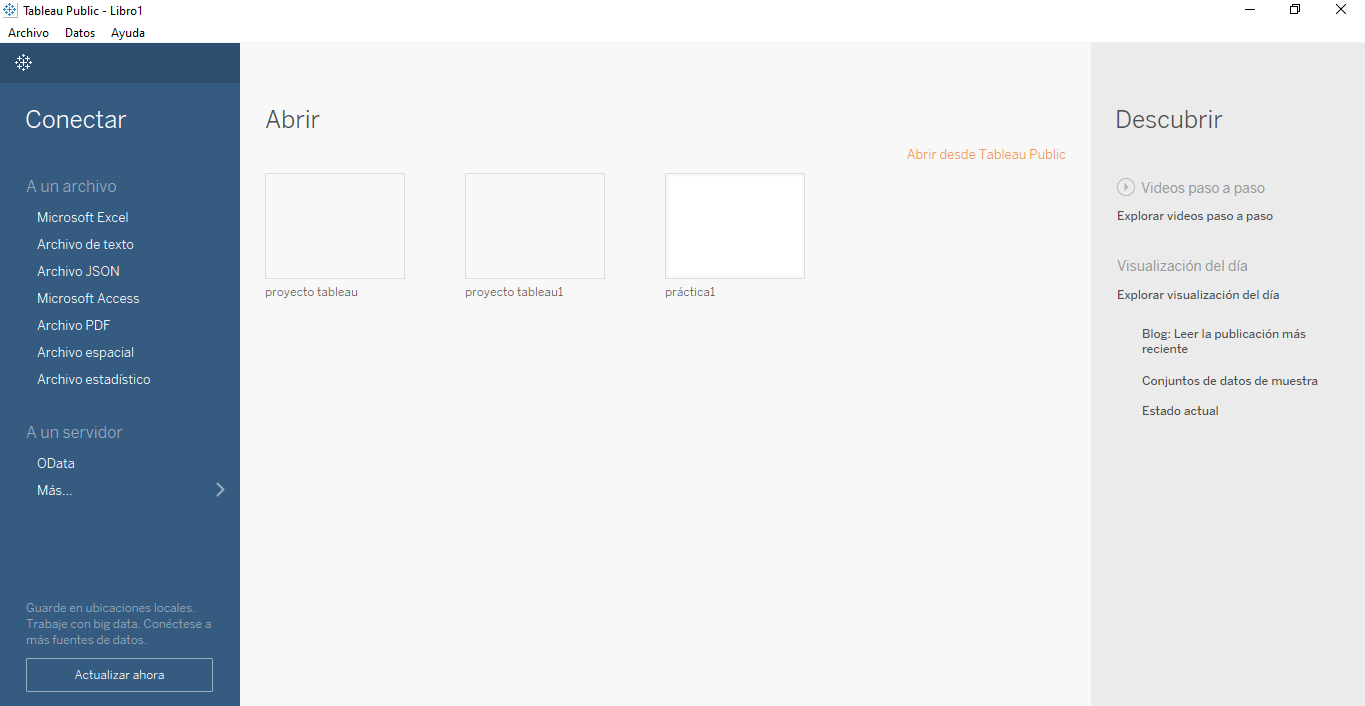
\includegraphics{imagenes/pr1.png}

\begin{enumerate}
\def\labelenumi{\arabic{enumi}.}
\tightlist
\item
  En la parte superior debajo del título \textbf{\emph{Conectar y A un
  archivo,}} seleccione Microsoft excel, debe realizar lo mismo como si
  estuviese abriendo un documento en el programa de Excel o Word. La
  lógica es la misma.
\item
  Se cargarán la base de datos
\item
  Debe arraztrar compañias al interfaz establecer conecciones, más aún
  si la base de datos tiene más de una hoja de excel.
\end{enumerate}

Ahora, se podrá ir a la hoja de trabajo. Antes de comenzar a realizar
las gráficas, se realiza una limpieza a la base de datos en cuanto a
formato u otros.

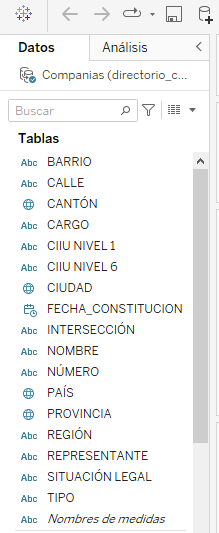
\includegraphics{imagenes/pr2.png}

\hypertarget{mostrarme}{%
\subsection{Mostrarme}\label{mostrarme}}

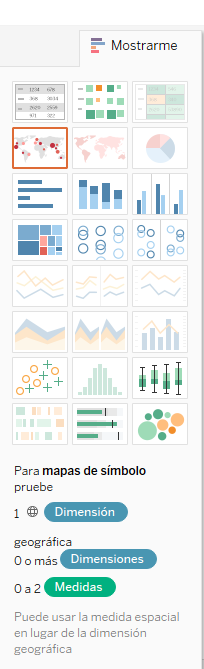
\includegraphics{imagenes/pr5.png}

La sección \textbf{Mostrarme} es una sección poderosa que facilita la
exploración y el análisis de datos de manera dinámica. Permite escoger y
visualizar ciertos campos y medidas. Al activar esta función, Tableau
sugiere automáticamente tipos de gráficos relevantes y transformaciones
de datos. Los gráficos se activan conforme cumplan los requerimientos
que se detallan en la parte inferior de la imagen.

\hypertarget{uso-del-calculate}{%
\subsection{Uso del CALCULATE}\label{uso-del-calculate}}

Una vez hecho, para obtener el total de empresas activas por periodo se
procedio:

\begin{enumerate}
\def\labelenumi{\arabic{enumi}.}
\tightlist
\item
  \textbf{Hacer un calculate}: para utilizar la función
  \textbf{\texttt{CALCULATE}} permite crear una fórmula calculada en
  Tableau. Para hacerlo, haz clic con el botón derecho del ratón en el
  área ``Dimensiones'' o ``Medidas'' del lienzo de trabajo y selecciona
  ``Crear campo calculado''. Esto abrirá el editor de fórmulas.
\item
  \textbf{Escribe tu Cálculo con CALCULATE:} En el editor de fórmulas,
  puedes escribir tu cálculo utilizando la función
  \textbf{\texttt{CALCULATE}} junto con otras funciones y campos de
  datos.
\end{enumerate}

En este caso se requiere conocer el total de empresas activas. En el
editor de fórmulas se detalla los códigos:

\texttt{\{WINDOW\_SUM(COUNT({[}SITUACIÓN\ LEGAL{]}\ =\ \textquotesingle{}ACTIVA\textquotesingle{}))\}}

\begin{enumerate}
\def\labelenumi{\arabic{enumi}.}
\item
  \textbf{\texttt{COUNT({[}SITUACIÓN\ LEGAL{]}\ =\ \textquotesingle{}ACTIVA\textquotesingle{})}}:
  Esta parte de la fórmula cuenta las filas donde la columna
  \textbf{\texttt{{[}SITUACIÓN\ LEGAL{]}}} tiene el valor `ACTIVA'. En
  otras palabras, está contando el número de registros donde la
  situación legal es `ACTIVA'. La empresa se encuentra en
  funcionamiento.
\item
  \textbf{\texttt{\{WINDOW\_SUM(...)\}}}: El resultado del paso anterior
  se utiliza como entrada para la función \textbf{\texttt{WINDOW\_SUM}}.
  Esta función se utiliza para realizar un cálculo de suma a lo largo de
  una ventana o un conjunto de registros. La ventana en este contexto
  generalmente se refiere a una vista de datos específica, como una
  tabla de datos en Tableau.
\end{enumerate}

Entonces, en resumen, esta fórmula cuenta cuántas veces aparece `ACTIVA'
en la columna \textbf{\texttt{{[}SITUACIÓN\ LEGAL{]}}} y luego realiza
una suma acumulativa de esa cantidad. El resultado será un valor
numérico que representa la suma acumulativa de empresas con situación
legal `ACTIVA' en la ventana de datos en la que se aplica esta fórmula.

Con ello, se obtiene el total de empresas activas hasta la fecha. Además
se puede obtener información de cuántas empresas se crearon en la
pandemia y despues de esta. Es así que procedemos a realizar otros
\textbf{\texttt{CALCULATE:}}

\texttt{SUM(\ IF\ {[}SITUACIÓN\ LEGAL{]}\ =\ \textquotesingle{}Activa\textquotesingle{}\ AND\ {[}FECHA\_CONSTITUCION{]}\ \textgreater{}=\ \#2020-02-29\#\ AND\ {[}FECHA\_CONSTITUCION{]}\ \textless{}=\ \#2023-05-05\#\ THEN\ 1\ ELSE\ 0\ END)}

Entonces \textbf{\texttt{SUM(...)}}: Es el comando principal que calcula
la suma total de los valores que cumplan con las condiciones
especificadas.

\begin{enumerate}
\def\labelenumi{\arabic{enumi}.}
\item
  \textbf{\texttt{IF\ {[}SITUACIÓN\ LEGAL{]}\ =\ \textquotesingle{}Activa\textquotesingle{}\ AND\ {[}FECHA\_CONSTITUCION{]}\ \textgreater{}=\ \#2020-02-29\#\ AND\ {[}FECHA\_CONSTITUCION{]}\ \textless{}=\ \#2023-05-05\#\ THEN\ 1\ ELSE\ 0\ END}}:
  Esta parte es una expresión condicional. Lo que está haciendo es lo
  siguiente:

  \begin{itemize}
  \item
    Comprueba si la columna \textbf{\texttt{{[}SITUACIÓN\ LEGAL{]}}} es
    igual a `Activa'.
  \item
    Comprueba si la columna \textbf{\texttt{{[}FECHA\_CONSTITUCION{]}}}
    es igual o posterior al 29 de febrero de 2020 y al mismo tiempo, es
    igual o anterior al 5 de mayo de 2023.
  \item
    Si ambas condiciones se cumplen, asigna el valor 1, de lo contrario,
    asigna el valor 0.El resultado de la expresión condicional es una
    serie de 1 y 0, donde 1 indica que una fila cumple con todas las
    condiciones y 0 indica que no las cumple.
  \end{itemize}
\end{enumerate}

Esto significa que suma todos los 1 y 0 según las filas que cumplan o no
cumplan las condiciones. El resultado final es la suma total de las
filas que cumplen todas las condiciones especificadas.

Lo mismo, se procede para obtener el total de empresas activas
pospandemia:

\texttt{SUM(IF\ {[}SITUACIÓN\ LEGAL{]}\ =\ \textquotesingle{}ACTIVA\textquotesingle{}\ AND\ {[}FECHA\_CONSTITUCION{]}\ \textgreater{}=\ \#2023-05-05\#\ THEN\ 1\ ELSE\ 0\ END)}

Para crear un gráfico, arrastra la expresión calculada al estante de
filas o columnas en la vista de hoja de trabajo y selecciona el tipo de
gráfico que mejor represente tus datos, como barras, líneas o
dispersión. Tableau aplicará automáticamente el cálculo a tus datos y
generará el gráfico correspondiente.'' En este contexto, la utilización
de un gráfico de barras resulta altamente eficaz para representar los
datos, especialmente cuando estos abarcan períodos cortos y presentan
variaciones significativas.

Por otro lado para obtener el promedio del capital suscrito de las
empresas activas se utiliza un \textbf{\texttt{CALCULATE}} siguiendo los
pasos explicados.

\texttt{AVG(IF\ {[}SITUACIÓN\ LEGAL{]}\ =\ \textquotesingle{}activa\textquotesingle{}\ THEN\ {[}CAPITAL\ SUSCRITO{]}\ END)}

El \textbf{AVG} permite obtener el promedio de un conjunto de datos.

Esta fórmula calcula el promedio de los valores de ``CAPITAL SUSCRITO''
únicamente para las empresas o registros que tienen una ``SITUACIÓN
LEGAL'' activa. Los valores que no cumplen con la condición de tener
``SITUACIÓN LEGAL'' igual a `activa' se excluyen del cálculo del
promedio (Esto se explico en el anterior punto sobre el uso del IF), lo
cual permite analizar el promedio del capital suscrito específicamente
para las empresas con una situación legal activa en un conjunto de
datos.

De igual forma con la mediana que es una medida estadística que se
utiliza para encontrar el valor que se encuentra en el centro de un
conjunto de datos cuando estos se organizan en orden ascendente o
descendente.:

\texttt{MEDIAN(IF\ {[}SITUACIÓN\ LEGAL{]}\ =\ \textquotesingle{}activa\textquotesingle{}\ THEN\ {[}CAPITAL\ SUSCRITO{]}\ END)}

Y asi con el quartil

\texttt{PERCENTILE({[}CAPITAL\ SUSCRITO{]},\ 0.2)}

La función \textbf{PERCENTILE} toma dos argumentos: el primer argumento
es el campo de datos del cual quieres encontrar el percentil, en este
caso, ``CAPITAL SUSCRITO''. El segundo argumento es el percentil que
deseas calcular, expresado como un número decimal. En este caso, es 0.2,
lo que significa que estás buscando el percentil 20.

\hypertarget{filtros}{%
\subsection{Filtros}\label{filtros}}

Para configurar un filtro en Tableau, primero arrastra la dimensión o
medida al estante de filtros, lo que abrirá una ventana emergente de
configuración. Aquí, puedes definir los valores que deseas mostrar,
elegir entre opciones como lista desplegable o menú de selección
múltiple, y personalizar el filtro.

Cabe mencionar que las opciones van a depender de la naturaleza de la
variable como se observa en la siguiente gráfica para una númerica:

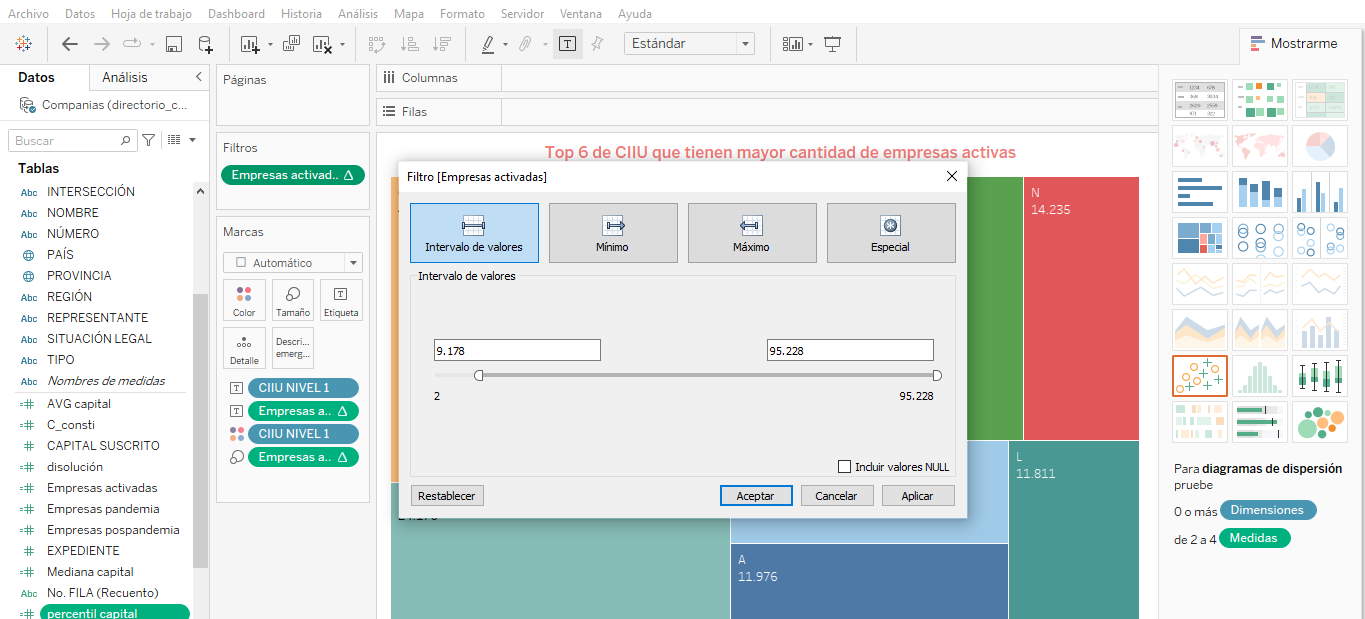
\includegraphics{imagenes/pr3.png}

Se le da un rango para poder obtener un top. En esta parte se utilizó un
treeplot, gráficos muy dinámicos que permite visualizar de forma
innovadora la información.

En cambio, en una variable cualitativa también podrás seleccionar solo
las categorias que se desea analizar en este caso como se muestra a
continuación:

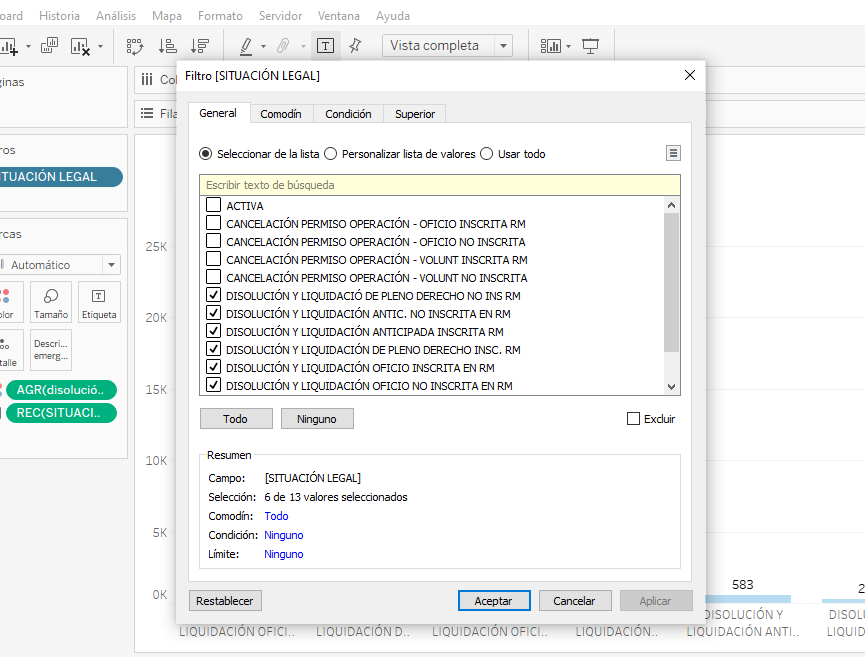
\includegraphics{imagenes/pr7.png}

\hypertarget{marcas}{%
\subsection{Marcas}\label{marcas}}

Esta sección te permite controlar cómo se visualizan y se representan
los datos en un gráfico específico. Es donde tomas decisiones clave
sobre la apariencia y el comportamiento de tus datos.

En \textbf{Marcas} hay diversas opciones que permite personalizar los
gráficos:

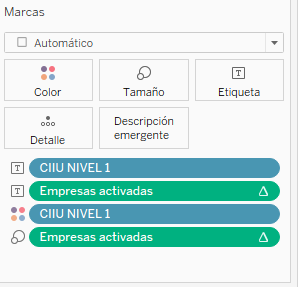
\includegraphics{imagenes/pr4.png}

\textbf{Color:} Controla los colores de las marcas en tu gráfico, es
útil para codificar información o categorizar tus datos visualmente por
colores.

\textbf{Tamaño:} Esta opción permite ajustar el tamaño de las marcas en
función de un campo de datos específico para resaltar la importancia o
cantidad de datos en cada marca.

\textbf{Etiqueta:} Aquí se puede especificar qué campo de datos se
utilizará para etiquetar las marcas directamente en la visualización.
Esto proporciona información adicional sin necesidad de hacer clic en
las marcas.

\textbf{Detalle:} Permite agregar campos de datos adicionales que se
mostrarán en la descripción emergente cuando pases el cursor sobre una
marca. Esto brinda detalles adicionales sin abrumar el gráfico
principal.

\textbf{Descripción emergente:} Te permite personalizar qué información
se muestra cuando se coloca el cursor sobre una marca en el gráfico.
Puedes incluir datos específicos y contexto adicional.

\hypertarget{mapa}{%
\subsection{Mapa}\label{mapa}}

Para hacer uso de los mapas debo tener variables geográficas, estas
permitirán que Tableau obtengan las coordenadas, seguidamente debo
seleccionar en la sección \textbf{Mostrarme} el gráfico del mapa.

\end{document}
